\chapter{Design Option Diagrams}
\label{designOptionsDiagrams}

\begin{figure}[!ht]
\centering
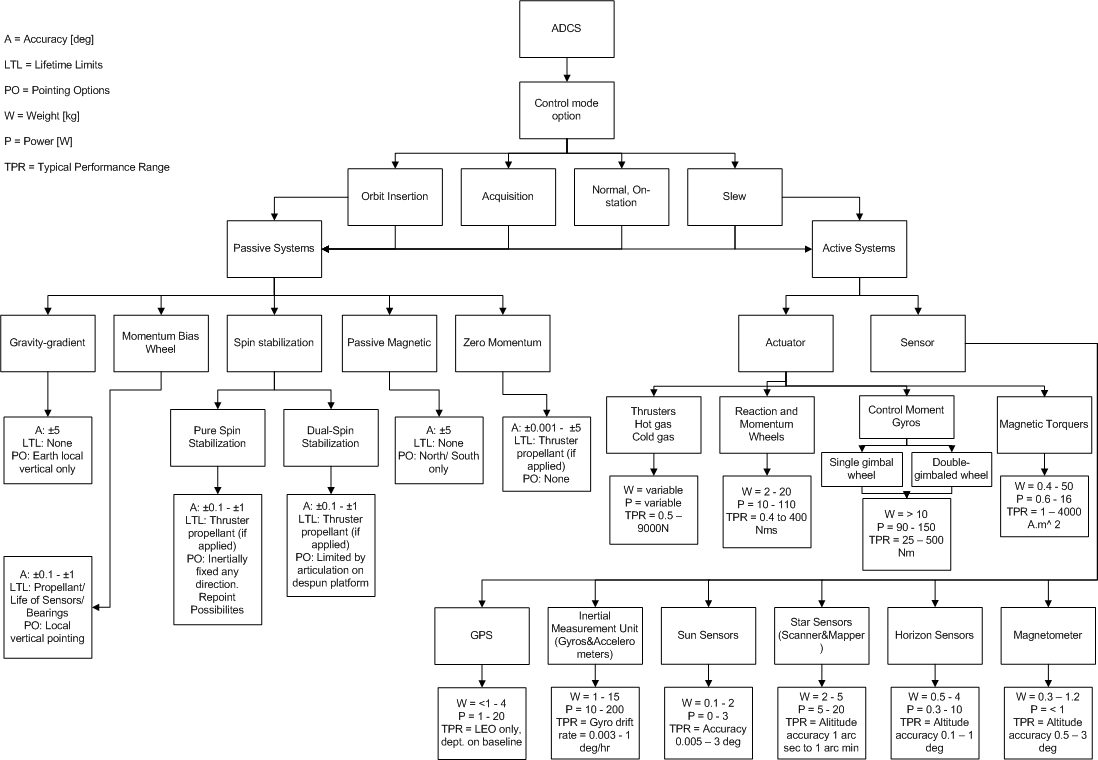
\includegraphics[width=0.9\textheight, angle=90]{chapters/img/DOTadcs.png}
\caption{Design option tree for the \ac{ADCS}}
\label{pic_DOTadcs}
\end{figure}

\begin{figure} [ht!]
	\centering
	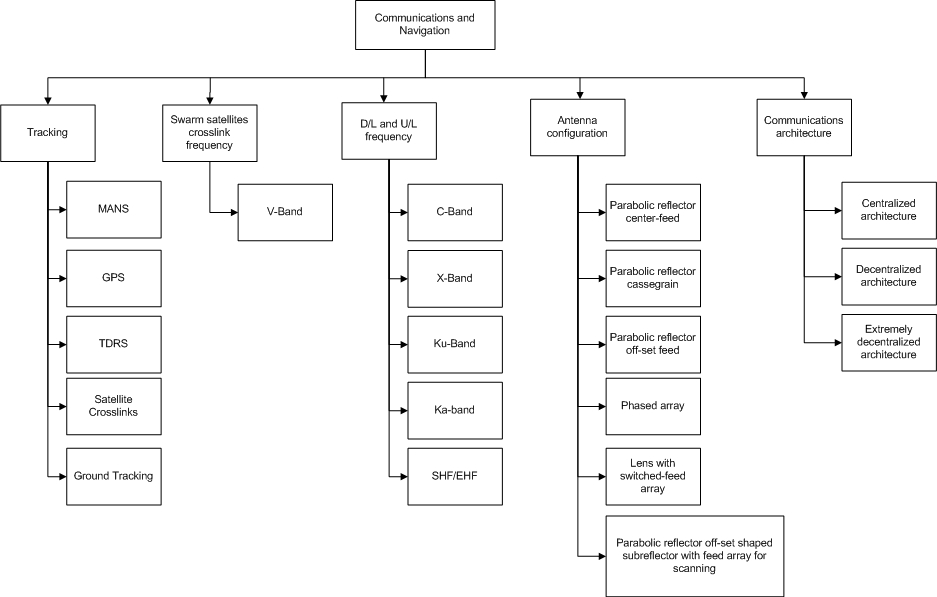
\includegraphics[width=0.9\textheight,angle=90]{chapters/img/DOTCom.jpg}	
	\caption{Design option tree for the communication systems}
	\label{fig:DOCom}
\end{figure}

\begin{figure}
\centering
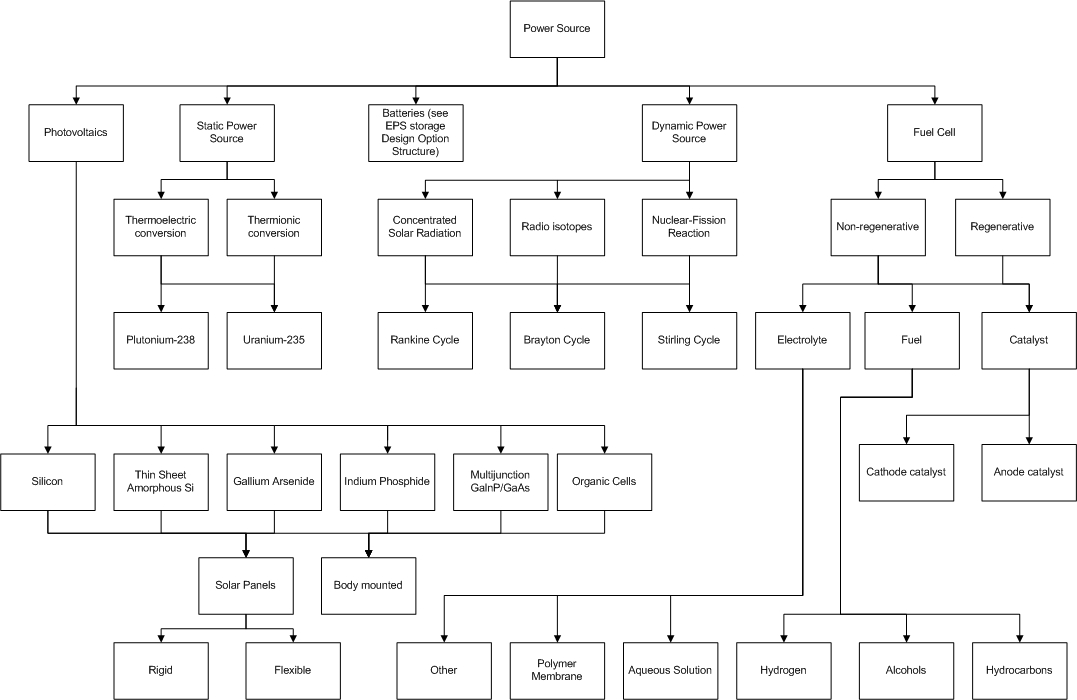
\includegraphics[width=1.0\textwidth, angle=90]{chapters/img/DOTeps_source.jpg}
\caption{Design option tree for the power source}
\label{pic_DOTeps_source}
\end{figure}

\begin{figure}
\centering
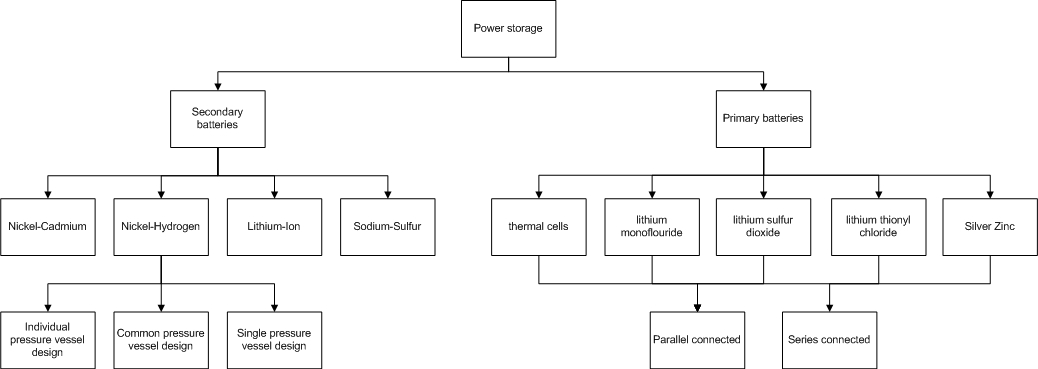
\includegraphics[width=1.0\textwidth, angle=90]{chapters/img/DOTeps_storage.jpg}
\caption{Design option tree for the power storage}
\label{pic_DOTeps_storage}
\end{figure}

\begin{figure} [ht]
\begin{center}
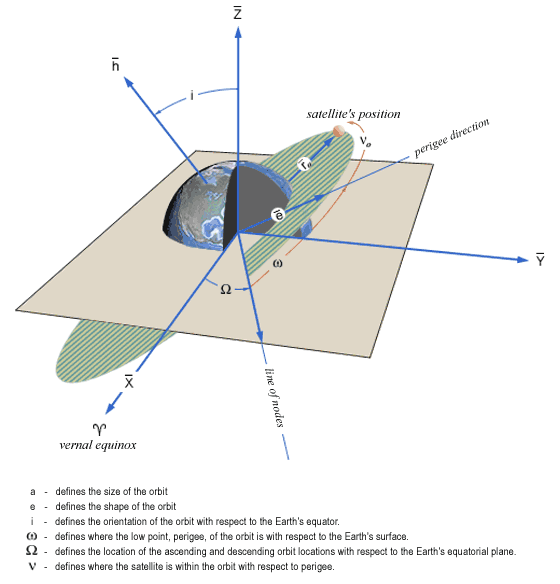
\includegraphics[width=0.75\textwidth,angle=0]{chapters/img/OrbElements.png}
\caption{Definitions of the inclination $i$, the right ascension of the ascending node $\Omega$, the argument of perigee $\omega$ and the true anomaly $\nu$. \emph{source: http://reentrynews.aero.org}}
\label{OrbElements}
\end{center}
\end{figure}

\begin{figure}
\centering
  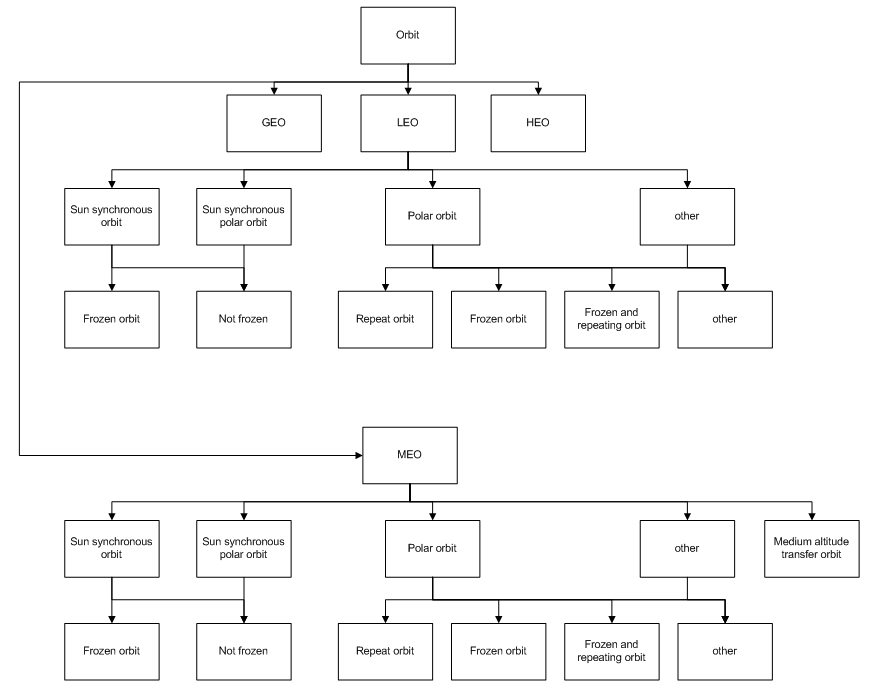
\includegraphics[width=0.75\textwidth,angle=0]{chapters/img/blDOOrb1.jpg}
	\caption{Design option tree for the orbit architecture of LEO and MEO}
	\label{DOOrb1}
\end{figure}

\begin{figure}
\centering
  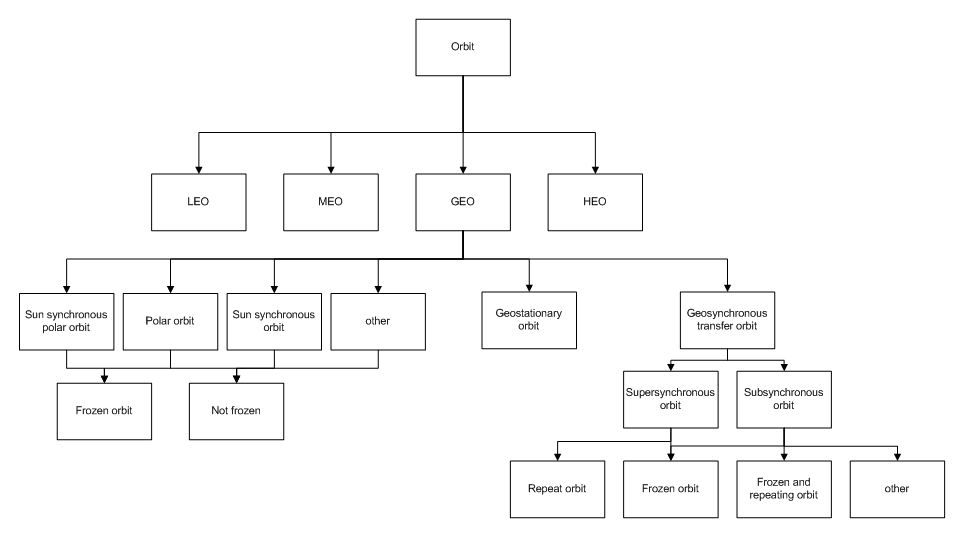
\includegraphics[width=0.75\textwidth,angle=0]{chapters/img/blDOOrb2.jpg}
	\caption{Design option tree for the orbit architecture of \ac{GEO}}
	\label{DOOrb2}
\end{figure}

\begin{figure}
\centering
  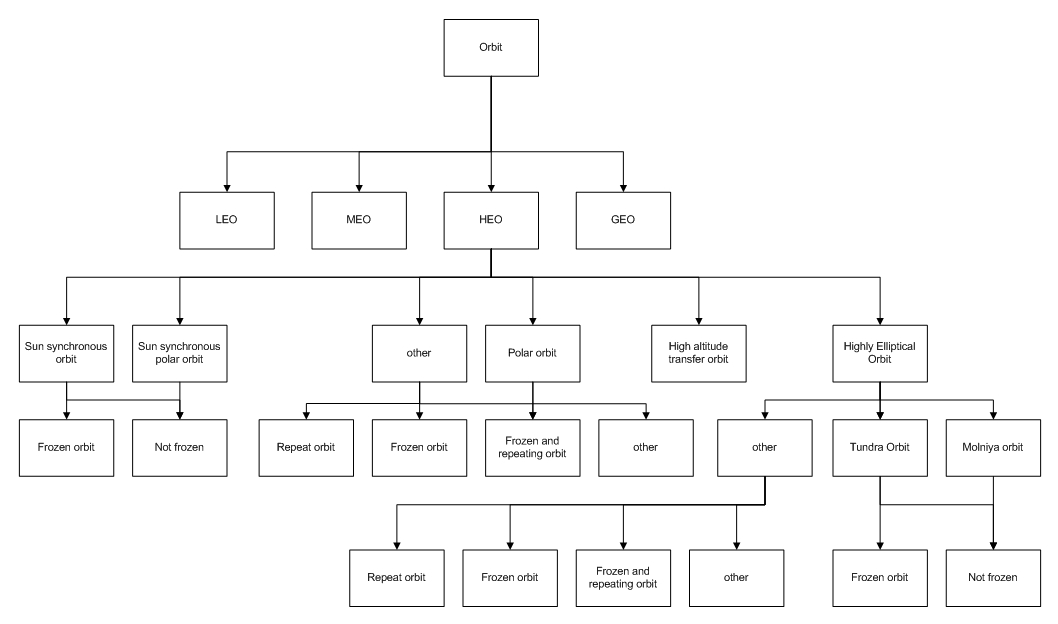
\includegraphics[width=0.75\textwidth,angle=0]{chapters/img/blDOOrb3.jpg}
	\caption{Design option tree for the orbit architecture of \ac{HEO}}
	\label{DOOrb3}
\end{figure}

\begin{figure}
\centering
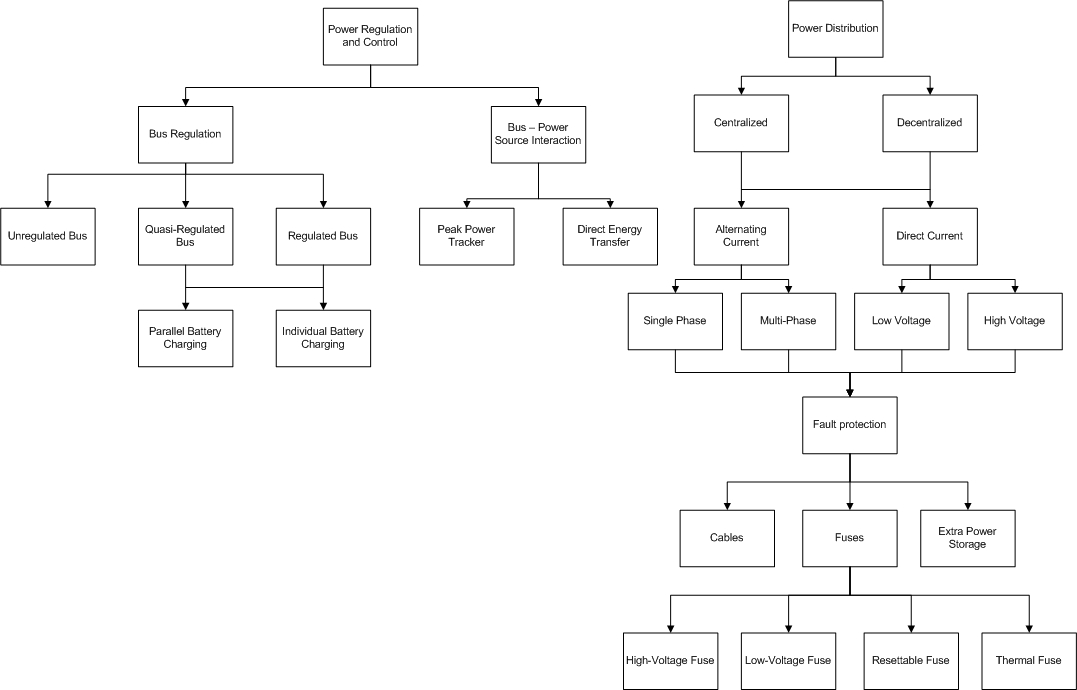
\includegraphics[width=1.0\textwidth, angle=90]{chapters/img/DOTeps_reganddis.jpg}
\caption{Design option tree for the distribution and regulation and control of the \ac{EPS}}
\label{pic_DOTeps_reganddis}
\end{figure}

\begin{figure} [!ht]
	\centering
	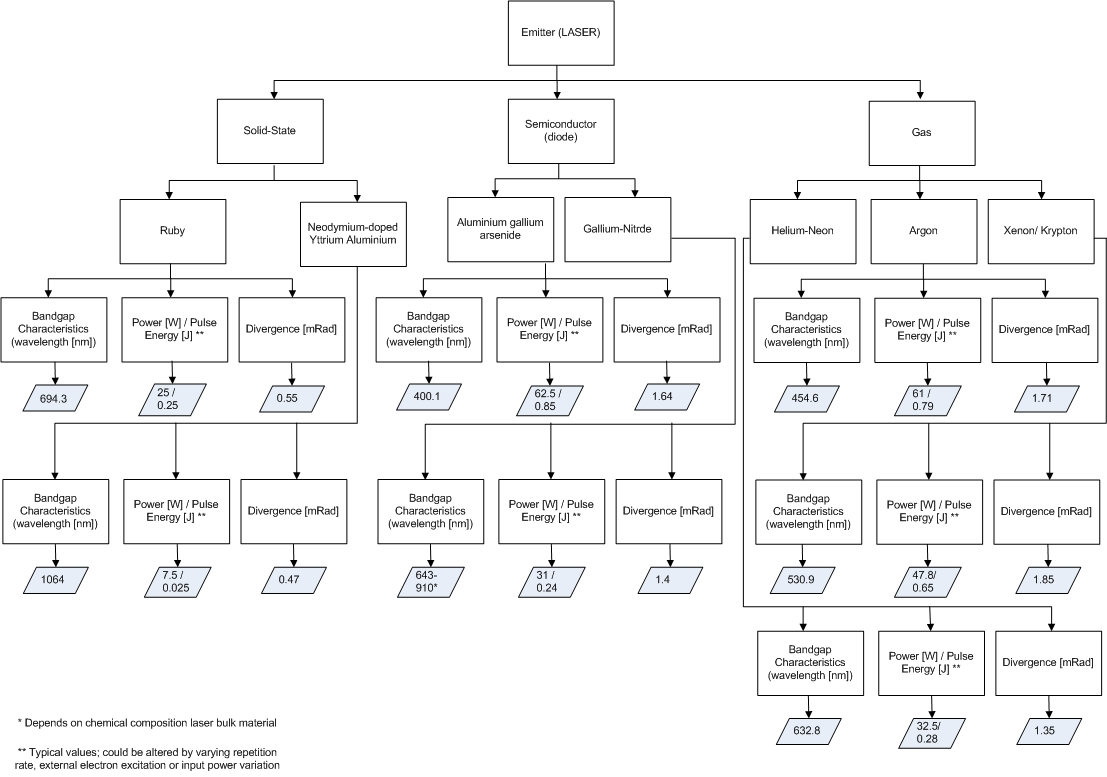
\includegraphics[height=0.85\textwidth,angle=90]{chapters/img/DOStree_laser.jpg}	
	\caption{Design option tree of laser emitter. Numbers indicate typical values.}
	\label{DOS_laser}
\end{figure}

\begin{figure} [ht]
\begin{center}
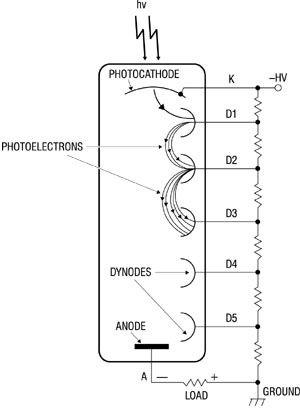
\includegraphics[scale=3]{chapters/img/DO_receiver1.jpg}	
\caption{Photomultiplier tube configuration and working mechanism}
\label{Photomultiplier}
\end{center}
\end{figure}

\begin{figure} [ht]
\begin{center}
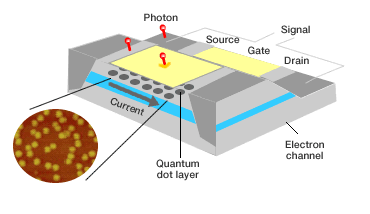
\includegraphics[scale=1]{chapters/img/blDOreceiverQDRD.png}	
\caption{Single photon detection using quantum dot configuration}
\label{quantumdot}
\end{center}
\end{figure}

\begin{figure} [ht]
\begin{center} 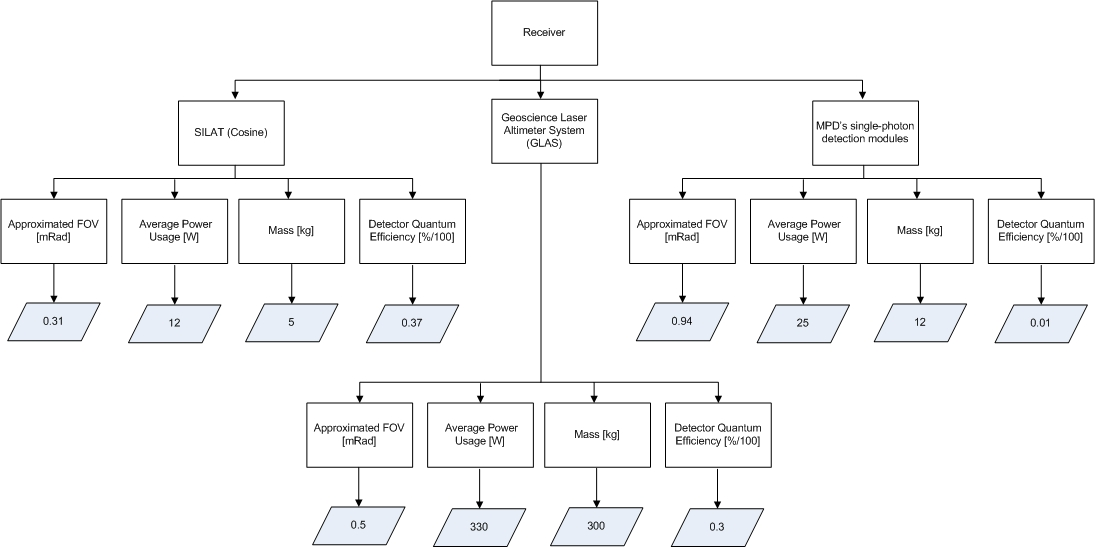
\includegraphics[width=1\textwidth,angle=90]{chapters/img/DOStree_receiver.jpg}	
\caption{Design option tree for laser receiver. Numbers represent typical values.}
\label{DOS_receiver}
\end{center}
\end{figure}